\section{Sistemi retroazionati: il luogo delle radici}


Il guadagno ad anello $L(s)$ di una funzione di trasferimento è descritto come:
\begin{equation}
  L(s) := K_1 \frac{
    (s-z_1)(s-z_2)\dots(s-z_m)
  }{
    (s-p_1)(s-p_2)\dots(s-p_n)
  }
\end{equation}

L'equazione caratteristica del sistema in retroazione è:
\begin{equation}
  1 + K_1 G_1(s) = 0
\end{equation}

Dove $G_1(s)$ è la funzione di trasferimento del sistema in retroazione.

\subsection{Il luogo delle radici}
\begin{definition}[Luogo delle radici diretto]
  Luogo delle radici (diretto) è il luogo geometrico descritto dalle radici 
  dell'equazione  $1 + K_1 G_1(s) = 0$ al variare di $K_1$ da $0^+$ a $+\infty$.
\end{definition}


\begin{definition}[Luogo delle radici inverso]
  Luogo delle radici (diretto) è il luogo geometrico descritto dalle radici 
  dell'equazione  $1 + K_1 G_1(s) = 0$ al variare di $K_1$ da $0^-$ a $-\infty$.
\end{definition}

\subsection{Proprità del luogo delle radici}
\begin{definition}[Proprietà 1]
  Il luogo ha tanti rami quanti sono i poli di $G_1(s)$.
  Ogni ramo parte da un polo e tende ad un zero o in un punto all'infinito.
  I rami si intersecano in in corrispondenza delle radici doppie.
\end{definition}

\begin{definition}[Proprietà 2]
  Il luogo delle raici è simmetrico rispetto all'asse reale.
\end{definition}


\begin{definition}[Proprietà 3]
  Nel luogo delle radici diretto, un punto dell'asse reale fa parte del luogo 
  se si lascia alla sua destra un numero dispari di poli e zeri.

  Nel luogo delle radici inverso, un punto dell'asse reale fa parte del luogo 
  se si lascia alla sua destra un numero pari di poli e zeri.
\end{definition}


\begin{figure}[h!]
  \centering
  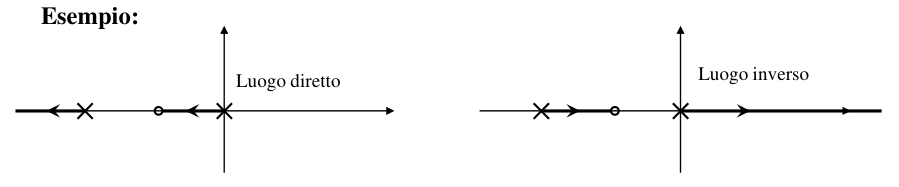
\includegraphics[width=0.8\linewidth]{./images/luogo_diretto_inverso.png}
  \caption{Luogo delle radici diretto e inverso}
  \label{fig:luogo_diretto_inverso}
\end{figure}



\subsection{Angoli di partenza e arrivo nel luogo}

\begin{definition}[Proprietà 4]
  Nel luogo delle radici \textbf{diretto} l'angolo di partenza da un polo $p_i$ semplice
  è definito come:
  \begin{equation}
    \text{angolo di partenza} = \varphi_i = \pi + \sum_{j=1}^m \arg (p_i - z_j) - \sum_{j=1, j\neq i}^n \arg (p_i - p_j)
  \end{equation}

  L'angolo di arrivo in un zero $z_i$ semplice è definito come:
  \begin{equation}
    \text{angolo di arrivo} = \psi_i = \pi + \sum_{j=1}^n \arg (z_i - p_j) - \sum_{j=1, j\neq i}^m \arg (z_i - z_j)
  \end{equation}
\end{definition}



Se il polo $p_i$ è multiplo di ordine $h > 1$, l'angolo di partenza è:
\begin{equation}
  h \varphi_i = \pi + \sum_{j=1}^m \arg (p_i - z_j) - \sum_{j=1, j\neq i}^n \arg (p_i - p_j) \quad \mod 2\pi
\end{equation}

Per gli zeri si ha:
\begin{equation}
  h \psi_i = \pi + \sum_{j=1}^n \arg (z_i - p_j) - \sum_{j=1, j\neq i}^m \arg (z_i - z_j) \quad \mod 2\pi
\end{equation}



\begin{definition}[Proprietà 5]
  Una radice del luogo di molteplicità $h$ corrisponde a un punto comune ad 
  $h$ rami in cui oltre all'equazione $1 + K_1G_1(s) = 0$ sono soddisfatte
  le relazioni:
  \begin{equation}
    D^i G_1(s) = 0 \quad i = 1,2,\dots,h-1
  \end{equation}
\end{definition}



\begin{definition}[Corollario]
  Una radice doppia soddisfa le relazioni:
  \begin{equation}
    \sum_{i=1}^n \frac{1}{s-p_i} = \sum_{i=1}^m \frac{1}{s-z_i}
  \end{equation}
\end{definition}

\begin{definition}[Proprietà 6]
  In corrispondenza di una radice di molteplicità $h$ il luogo presenta $h$
  rami entranti ed $h$ rami uscenti alternati fra loro, le cui tangenti suddividono
  lo spazio circostante in settori uguali di $\pi/h$ radianti.
\end{definition}



\begin{definition}[Proprietà 7]
  Gli asintoti del luogo formano una stella di raggi con centro nel punto dell'asse
  reale di ascissa:
  \begin{equation}
    \sigma_a = \frac{\sum_{i=1}^n p_i - \sum_{i=1}^m z_i}{n-m}
  \end{equation}

  Se il luogo è \textbf{diretto} gli asintoti formano con l'asse reale gli angoli:
  \begin{equation}
    \theta_{a, v} = (2v+1)\frac{\pi}{n-m} \quad v = 0,1,2,\dots,n-m-1
  \end{equation}

  Se il luogo è \textbf{inverso} gli asintoit formano con l'asse reale gli angoli:
  \begin{equation}
    \theta_{a, v} = \frac{2v\pi}{m-n} \quad v = 0,1,2,\dots,m-n-1
  \end{equation}
\end{definition}


\begin{figure}[h!]
  \centering
  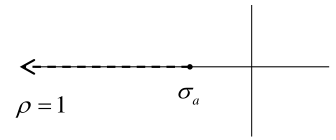
\includegraphics[width=0.3\linewidth]{./images/luogo_diretto_rho_1.png}
  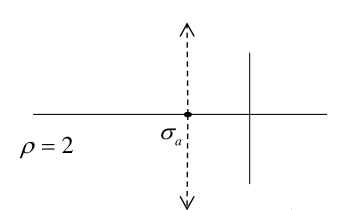
\includegraphics[width=0.3\linewidth]{./images/luogo_diretto_rho_2.png}
  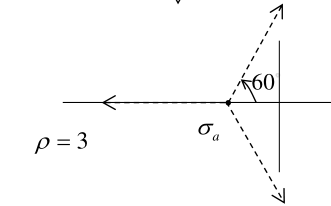
\includegraphics[width=0.3\linewidth]{./images/luogo_diretto_rho_3.png}
  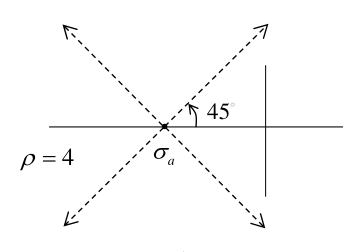
\includegraphics[width=0.3\linewidth]{./images/luogo_diretto_rho_4.png}
  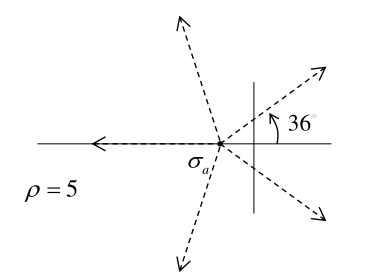
\includegraphics[width=0.3\linewidth]{./images/luogo_diretto_rho_5.png}
  \caption{Esempi di luoghi diretti con diverse molteplicità}
  \label{fig:luogo_diretto}
\end{figure}


\begin{figure}[h!]
  \centering
  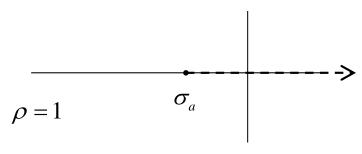
\includegraphics[width=0.3\linewidth]{./images/luogo_inverso_rho_1.png}
  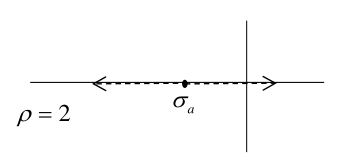
\includegraphics[width=0.3\linewidth]{./images/luogo_inverso_rho_2.png}
  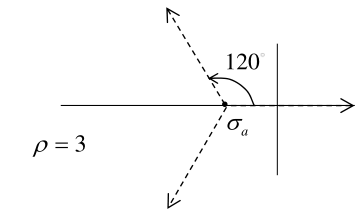
\includegraphics[width=0.3\linewidth]{./images/luogo_inverso_rho_3.png}
  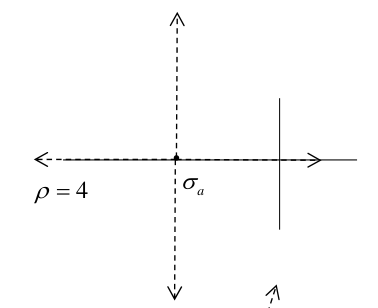
\includegraphics[width=0.3\linewidth]{./images/luogo_inverso_rho_4.png}
  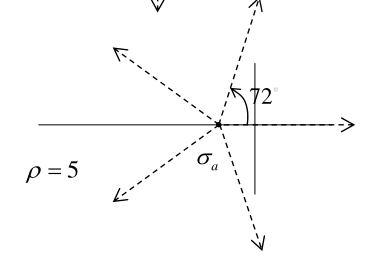
\includegraphics[width=0.3\linewidth]{./images/luogo_inverso_rho_5.png}
  \caption{Esempi di luoghi inversi con diverse molteplicità}
  \label{fig:luogo_inverso}
\end{figure}


\newpage
\subsection{Grado di stabilità}
\begin{definition}[Grado di stabilità]
  Si definisce grado di stabilità di $\sum$ (nel piano complesso):
  \begin{equation}
    G_s := - \max \{ \Re (p_i) \} \quad i = 1,2,\dots,n
  \end{equation}
\textbf{  È la disatanza minima dei poli di $\sum$ dall'asse immaginario.}

Se è presente una coppia dominante vale approssimare:
\begin{equation}
  T_a \approx \frac{3}{G_s}
\end{equation}
\end{definition}


